\chapter{LOGARITHM APPROXIMATION}
\label{chap:logarithm_approximation}
Many methods to compute transcendental functions implemented in computer hardware and software libraries rely on direct knowledge of the function arguments. Several such approaches include CORDIC (coordinate rotation digital computer), pseudo-division and pseudo-multiplication algorithms~\cite{walther_cordic_2000}, as well as minimax polynomials, which are determined numerically using the Remez algorithm~\cite{harrison_computation_1999}. These algorithms, while efficient, rely on table lookups, which cannot be done in a privacy-preserving system where the function arguments cannot be directly determined.

We must therefore rely on other methods, such as using the Taylor series expansions of these functions. While also in common use, not all Taylor series expansions have a convenient radius of convergence. To circumvent this, we can rely on an approach presented by Khattri in~\cite{khattri_new_2009} to obtain closed-form approximations to functions by approximating related integrals.

\section{Known Closed-Form Logarithm Approximations}
Khattri ~\cite{khattri_new_2009} presents the following method to approximate the function $f(x)=\log\left(1+x\right)$.
Let $x = 1/n$ and consider the integral
\begin{align}
	\label{eq:log_integral}
	\int_{n}^{n+1}{\frac{1}{t}\diff t}=\log{\left(1+\frac{1}{n}\right)}.
\end{align}

This integral can be approximated using the five-point Gauss--Legendre quadrature rule~\cite{kythe_quadrature_2002}. We first convert the integral to an integral over the interval $[-1,1]$ using the following transformation:
\begin{align*}
	\int_a^b{f(x)\diff x}
	&= \frac{b-a}{2}\int_{-1}^{1}{f\left(\frac{b-a}{2}x+\frac{a+b}{2}\right)\diff x}.
\end{align*}
Then, we approximate the integral using the following summation:
\begin{equation*}
	\int_{-1}^{1}{f\left(x\right)\diff x} \approx \sum_{i=1}^{5}{w_i f\left(x_i\right)},
\end{equation*}
where
\begin{multicols}{2}
	\noindent
	\begin{align*}
		w_1 &= 0,\\
		w_2 &= \frac{1}{21}\sqrt{245-14\sqrt{70}},\\
		w_3 &= -\frac{1}{21}\sqrt{245-14\sqrt{70}},\\
		w_4 &= \frac{1}{21}\sqrt{245+14\sqrt{70}},\\
		w_5 &= -\frac{1}{21}\sqrt{245+14\sqrt{70}},
	\end{align*}
	\columnbreak
	\begin{align*}
		x_1 &= \frac{128}{225},\\
		x_2 &= \frac{1}{900}\left( 322 + 13\sqrt{70}\right),\\
		x_3 &= \frac{1}{900}\left( 322 + 13\sqrt{70}\right),\\
		x_4 &= \frac{1}{900}\left( 322 - 13\sqrt{70}\right),\\
		x_5 &= \frac{1}{900}\left( 322 - 13\sqrt{70}\right).
	\end{align*}
\end{multicols}
Applying this procedure to the integral in Equation~\ref{eq:log_integral} yields the following approximation:
\begin{equation}\label{eq:standard_logarithm_quadrature}
	\log\left(1+x\right) \approx
	\frac{137x^5 + 2310x^4 + 9870x^3 + 15120x^2 + 7560x}
	{30x^5 + 900x^4 + 6300x^3 + 16800x^2 + 18900x + 7560}.
\end{equation}

While the closed-form approximation presented by Khattri (Equation~\ref{eq:standard_logarithm_quadrature}) is accurate for values of $x$ near zero, it diverges from $\log{\left(1+x\right)}$ significantly for large values of $x$, as shown in Figure~\ref{fig:standard_logarithm_quadrature}.
\begin{figure}[!ht]
	\centering
	% \begin{tikzpicture}
	% 	\begin{axis}[
	% 		% height=6cm, width=9cm,
	% 		xmin=0, xmax=300,
	% 		ymin=0, ymax=5.5, ytick={0,...,6},
	% 		xlabel={$x$}, ylabel={$y$},
	% 		grid=major,
	% 		legend pos=south east,
	% 		legend cell align=left,
	% 	]
	% 	\addplot[very thick, blue, domain=0:300, samples=100]{1/30*(137*x^5 + 2310*x^4 + 9870*x^3 + 15120*x^2 + 7560*x)/(x^5 + 30*x^4 + 210*x^3 + 560*x^2 + 630*x + 252)};
	% 	\addplot[densely dashed, domain=0:300, samples=100]{ln(x)};
	% 	\legend{5-point quadrature approximation, Actual value of $\log(1+x)$}
	% 	\end{axis}
	% \end{tikzpicture}%
    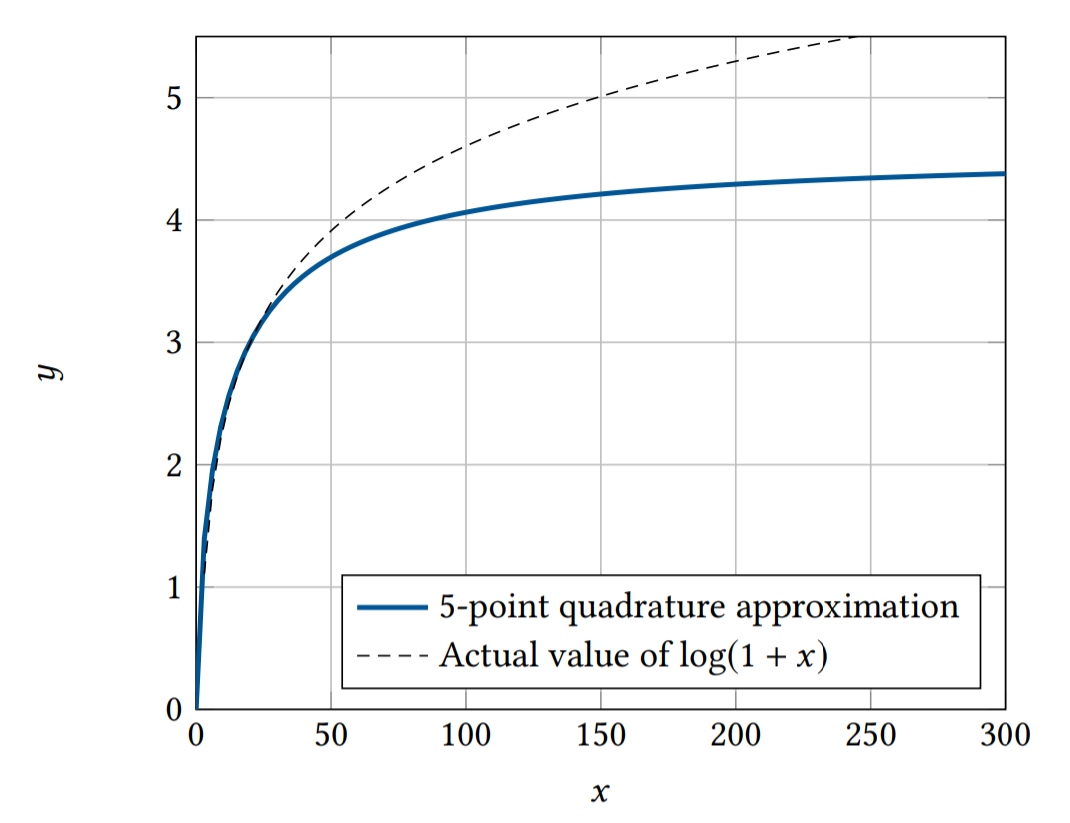
\includegraphics[width=12cm]{figures/graph_log_a2.png}
	\caption{Graph of $\log{\left(1+x\right)}$ and the approximation in Equation~\ref{eq:standard_logarithm_quadrature}}
	\label{fig:standard_logarithm_quadrature}
\end{figure}

However, the quadrature approach presented by Khattri allows us to approximate the logarithm in a larger range than is possible with the Taylor series, as the Taylor series of $\log\left(1+x\right)$ has an interval of convergence of $[-1,1]$.

\section{Scaled Approximation}
\label{sec:logarithm_approximation}
This appendix a general method to improve the general accuracy of the logarithm approximation given by Khattri in~\cite{khattri_new_2009} for use in privacy-preserving calculation, provided that accuracy is only required for a specific range.

For this approximation, we assume we only require accurate results in the input range $x \in [0, 255]$, to reflect use as part of the logarithm image transformation.

Since the approximation by Khattri is accurate for values of $x$ near zero, we can scale the approximation by a constant factor $\alpha$ by expressing $\log(1+x)$ as follows, similarly using the substitution $x=1/n$:
\begin{align*}
	\log{\left(1+x\right)} &= \log{\left(\frac{\alpha + \alpha x}{\alpha}\right)}\\
	&= \log{(\alpha + \alpha x)} - \log{\alpha}\\
	&= \log{\left(\alpha+\frac{\alpha}{n}\right)} - \log{\alpha}\\
	&= \log{\left(\frac{\alpha n + \alpha}{n}\right)} - \log{\alpha}\\
	&= \int_{n}^{\alpha n + \alpha}{\frac{1}{t}\diff t} - \log{\alpha}.
\end{align*}

Applying the five-point Gauss--Legendre quadrature rule to approximate $\int_{n}^{\alpha n + \alpha}{\frac{1}{t}\diff t}$ with $\alpha = 1/16$ using SageMath 8.3, we arrive at the approximation:
\begin{align}\label{eq:optimal_log_approximation}
	\begin{split}
		&\log\left(1+x\right) \\
		&\approx \frac{137x^5 + 26685x^4 + 617370x^3 - 6498630x^2 - 121239315x - 257804775}
		{30(x^5 + 405x^4 + 27210x^3 + 488810x^2 + 2536005x + 3122577)}\\
		&+ \log{16}.
	\end{split}
\end{align}

We note that the approximation in Equation~\ref{eq:optimal_log_approximation} requires the value of $\log{16}$. This can be computed in the plaintext domain and added to an encrypted value using the properties of the Paillier or DGK cryptosystems, while an FHE scheme would have to encrypt the value of $\log{16}$. The remaining arithmetic operations in the approximation can be computed in the encrypted domain, using the protocols described in Section~\ref{sec:fp_arithmetic}. Therefore, this approximation can be calculated in a privacy-preserving manner.

Figure~\ref{fig:log_error_comparison} is a graph comparing the absolute error of the scaled approximation and the original approximation by Khattri given an input $x$. We can see that scaling the input by some constant factor $\alpha$ improves the accuracy of the closed-form approximation, although it requires that $\log \alpha$ be known.

\begin{figure}[ht]
	\centering
  %   \begin{tikzpicture}
	% 	\begin{semilogyaxis}[
	% 		% height=6cm, width=9cm,
	% 		xmin=0, xmax=300,
	% 		ymin=1e-10, ymax=1.4,
	% 		xlabel={$x$}, ylabel={Absolute error},
	% 		grid=major,
	% 		legend pos=south east,
	% 		legend cell align=left,
	% 		tick scale binop=\times,
	% 	]
	% 	% \addplot[very thick, domain=0:300, samples=500]{abs(-1/30*(x^5*(30*ln(1/16) - 137) + 45*x^4*(270*ln(1/16) - 593) + 30*x^3*(27210*ln(1/16) - 20579) + 30*x^2*(488810*ln(1/16) + 216621) + 45*x*(1690670*ln(1/16) + 2694207) + 93677310*ln(1/16) + 257804775)/(x^5 + 405*x^4 + 27210*x^3 + 488810*x^2 + 2536005*x + 3122577) - ln(x + 1))};
	% 	% \addplot[very thick, domain=0:300, samples=300]{abs(1/30*(137*x^5 + 26685*x^4 + 617370*x^3 - 6498630*x^2 - 121239315*x - 257804775)/(x^5 + 405*x^4 + 27210*x^3 + 488810*x^2 + 2536005*x + 3122577) - ln(1/16) - ln(x + 1))};
	% 	\addplot[very thick, blue] table[x=x, y=error] {plots/abs_err_scaledlog.txt};
	% 	\addplot[densely dashed, domain=0:300, samples=100]{abs(1/30*(137*x^5 + 2310*x^4 + 9870*x^3 + 15120*x^2 + 7560*x)/(x^5 + 30*x^4 + 210*x^3 + 560*x^2 + 630*x + 252) - ln(x + 1))};
	% 	\legend{Scaled quadrature ($\alpha = 1/16$), Original quadrature ($\alpha = 1$)}
	% \end{semilogyaxis}
	% \end{tikzpicture}%
    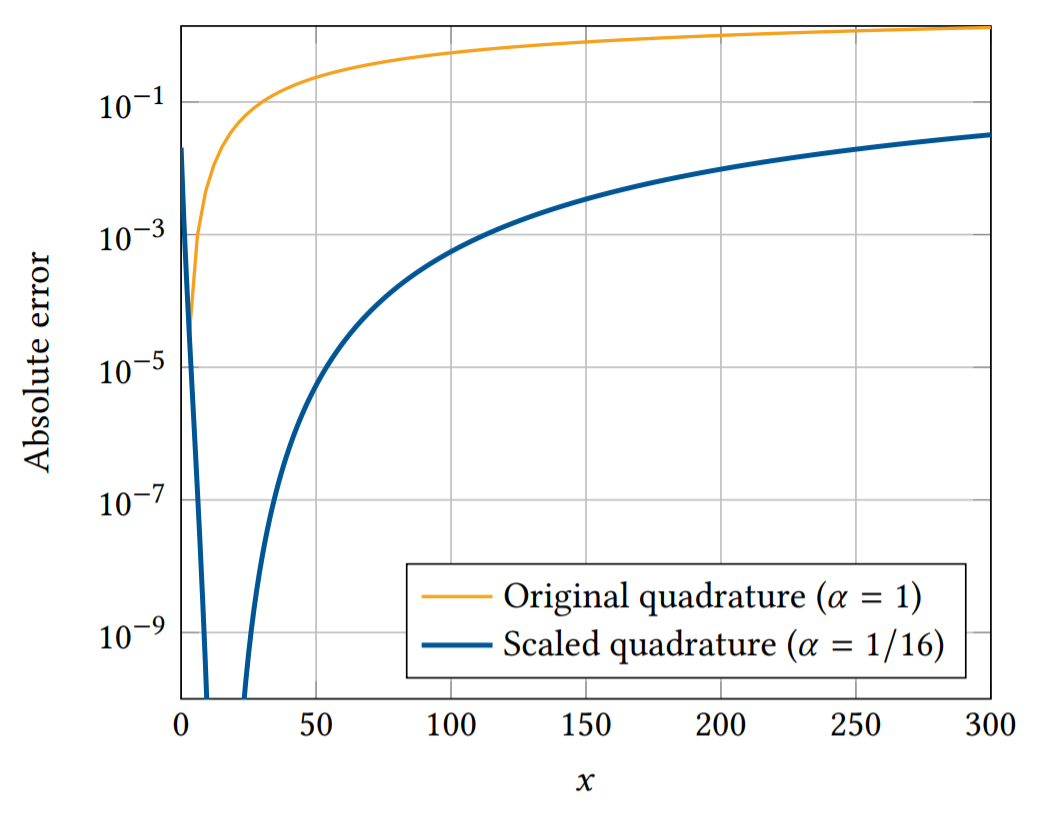
\includegraphics[width=12cm]{figures/comp_errs.png}
	\caption{Comparison of the absolute error between the original approximation in Equation~\ref{eq:standard_logarithm_quadrature} and the scaled approximation in Equation~\ref{eq:optimal_log_approximation}}
	\label{fig:log_error_comparison}
\end{figure}

We now show how we used numerical methods to determine that a scaling factor of $\alpha = 1/16$ minimizes the maximum absolute error of the scaled approximation for $\log{\left(1+x\right)}$, within the range $x \in [0, 255]$.

Let $I\left(x,\alpha\right)$ be the function obtained by approximating $\int_{n}^{\alpha n + \alpha}{\frac{1}{x}\diff x}$ with five-point Gauss--Legendre quadrature. The absolute error of the approximation compared to $\log{\left(1+x\right)}$ at a given $x$ and $\alpha$ is given by the following function.
\begin{align*}
	A\left(x,\alpha\right) = \left| I\left(x,\alpha\right) - \log\alpha - \log{\left(1+x\right)}\right|.
\end{align*}
We want to show that the function
\begin{align*}
	f\left(\alpha\right) = \max_{0\leq x \leq 255}{A\left(x,\alpha\right)}
\end{align*}
is minimized at $\alpha = 1/16$.
We consider the functions $A\left(0,\alpha\right)$ and $A\left(255,\alpha\right)$. These are plotted in Figure~\ref{fig:endpoint_plot}.
\begin{figure}[!ht]
	\centering
  %   \begin{tikzpicture}
	% 	\begin{semilogyaxis}[
	% 		% height=6cm, width=9cm,
	% 		xmin=0, xmax=1,
	% 		ymin=5e-7, ymax=1.3,
	% 		xlabel={$\alpha$}, ylabel={Absolute error},
	% 		grid=major,
	% 		extra x ticks={1/16},
	% 		extra x tick labels={$\frac{1}{16}$},
	% 		legend pos=south east,
	% 		legend cell align=left,
	% 		tick scale binop=\times,
	% 	]
	% 	\addplot[thick, ACMDarkBlue, domain=0:1] table[x=alpha, y=x0] {plots/abs_err_sl_0_255.txt};
	% 	\addplot[thick, ACMOrange, domain=0:1] table[x=alpha, y=x255] {plots/abs_err_sl_0_255.txt};
	% 	\legend{$x=0$, $x=255$}
	% 	% \legend{$A\left(0,\alpha \right)$, $A\left(255,\alpha \right)$}
	% \end{semilogyaxis}
	% \end{tikzpicture}%
    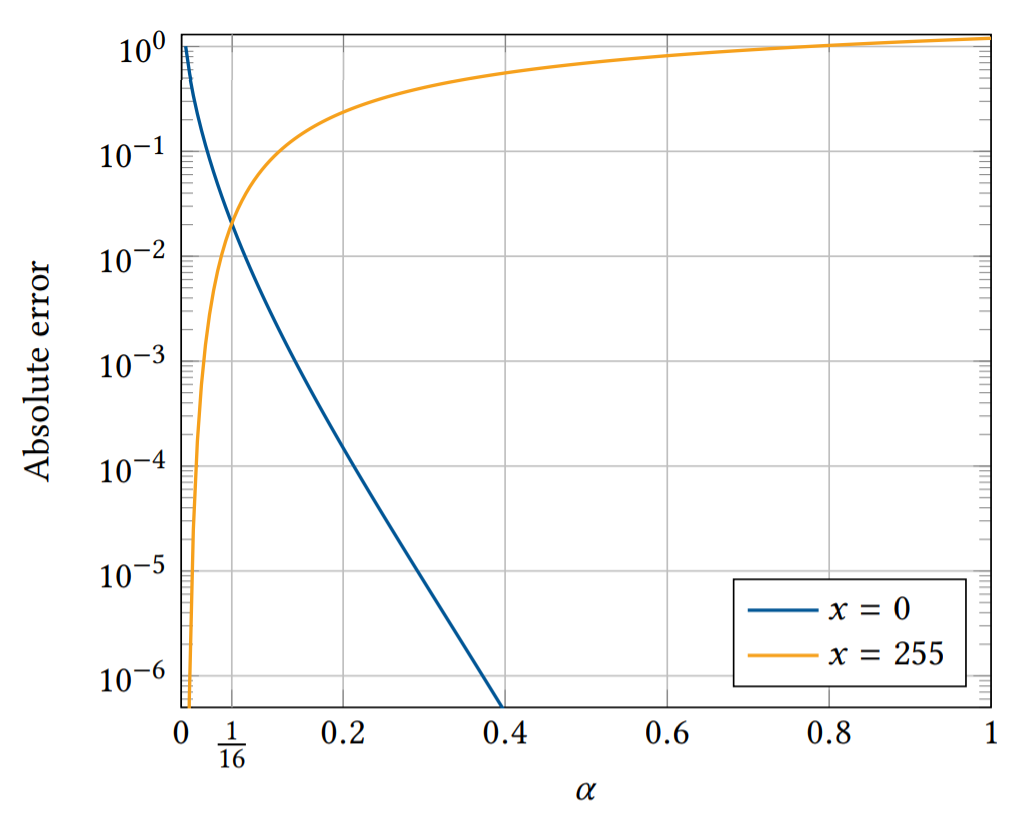
\includegraphics[width=12cm]{figures/graph_0_255.png}
	\caption{Graphs of $A\left(x,\alpha\right)$ at $x=0$ and $x=255$}
	\label{fig:endpoint_plot}
\end{figure}

It can be determined numerically using SageMath 8.3 that a local minimum of $\max\left(A\left(0,\alpha\right),A\left(255,\alpha\right)\right)$ on the interval $[0,1]$ is at $\alpha = 1/16$, which is found at the intersection of the two graphs.

We then consider the function $A\left(x,1/16\right)$, shown in Figure~\ref{fig:single_alpha_plot}.
It was determined numerically that the local maxima of $A\left(x,1/16\right)$ on the interval occur at $x=0$ and $x=255$. Since a scaling factor other than $\alpha=1/16$ yields a higher absolute error at either $x=0$ or $x=255$, as seen in Figure~\ref{fig:endpoint_plot}, it follows that a scaling factor of $\alpha = 1/16$ minimizes the maximum absolute error of the scaled approximation for $\log{\left(1+x\right)}$, within the range $x \in [0, 255]$.
\begin{figure}[ht]
	\centering
	% \begin{tikzpicture}
	% 	\begin{semilogyaxis}[
	% 		xmin=0, xmax=300,
	% 		ymin=1e-15, ymax=0.035,
	% 		xlabel={$x$}, ylabel={Absolute error},
	% 		grid=major,
	% 		legend pos=south east,
	% 		legend cell align=left,
	% 		tick scale binop=\times,
	% 	]
	% 	% \addplot[very thick, domain=0:300, samples=300]{abs(1/30*(137*x^5 + 26685*x^4 + 617370*x^3 - 6498630*x^2 - 121239315*x - 257804775)/(x^5 + 405*x^4 + 27210*x^3 + 488810*x^2 + 2536005*x + 3122577) - ln(1/16) - ln(x + 1))};
	% 	\addplot[thick, ACMDarkBlue] table[x=x, y=error] {plots/abs_err_scaledlog.txt};
	% \end{semilogyaxis}
	% \end{tikzpicture}%
    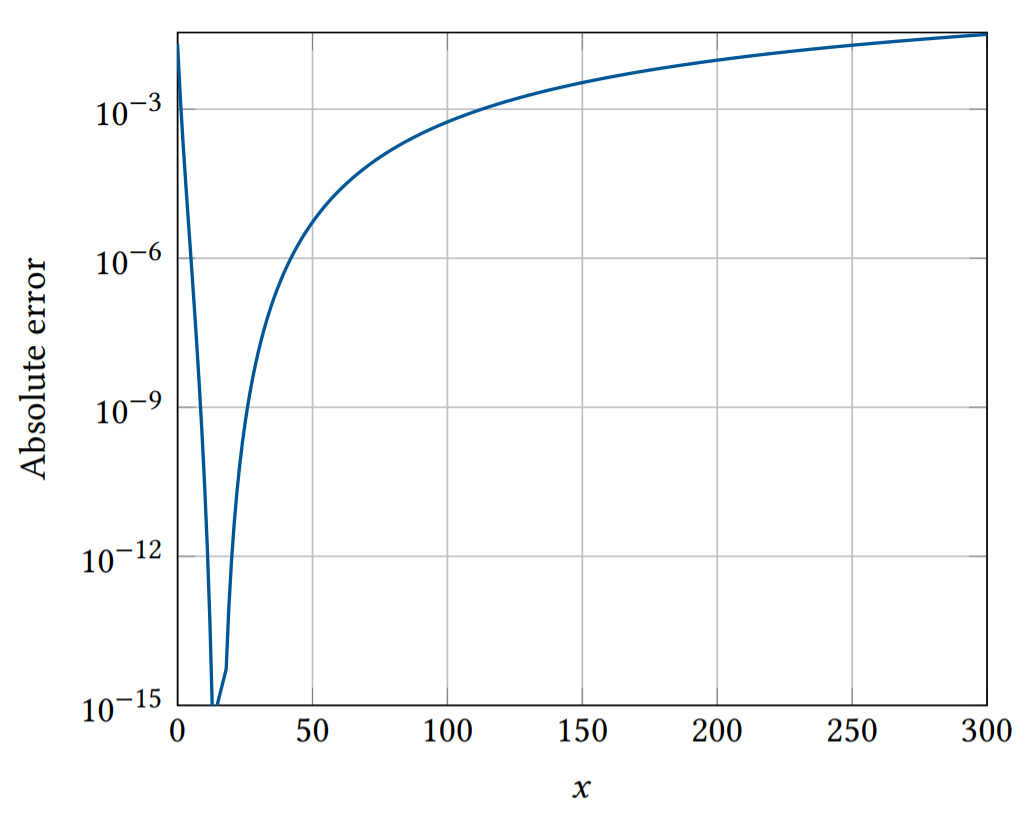
\includegraphics[width=12cm]{figures/graph_approx_16.png}
	\caption{Graph of $A\left(x,1/16\right)$, the absolute error of the approximation in Equation~\ref{eq:optimal_log_approximation} given a scaling factor of $\alpha=1/16$}
	\label{fig:single_alpha_plot}
\end{figure}

We have shown how we can adapt Khattri's approximation to allow for privacy-preserving logarithm computation over a larger interval.

\section{Approximation for $x^\gamma$}
To approximate $x^\gamma$ for any $\gamma \in \mathbb{R}$, we rewrite $x^\gamma$ as follows:
\begin{align*}
  x^\gamma = e^{\log{x^\gamma}} = e^{\gamma\log{x}}.
\end{align*}
This expression can then be approximated using the Maclaurin series expansion for $e^x$, which converges for all $x$.
\begin{align*}
  e^x &= \sum_{n=0}^{\infty}{\frac{x^n}{n!}}\\
  \Rightarrow e^{\gamma\log{x}} &= \sum_{n=0}^{\infty}{\frac{(\gamma\log{x})^n}{n!}}
\end{align*}
As we already have an approximation for the natural logarithm, we can evaluate partial sums of the above infinite series to arrive at approximations for $x^\gamma$.
